% coherence_mln_deepdive.tex
% Deep dive on the Markov Logic Network (MLN) formulation for logical coherence.
% Companion to coherence_mrf_deepdive.tex, coherence_modeling.tex, and research_plan.md;
% focuses ONLY on the MLN. Compile: pdflatex coherence_mln_deepdive.tex (run twice).
%
% All numeric weights / marginals / Z / MAP values are EXACT (brute force over 2^16
% worlds) for the AeroParts model. The MLN weights use w = logit(p) on the log-linear
% (three-clause) encoding, which reproduces the with-priors MRF exactly; the numbers
% therefore coincide with those in coherence_mrf_deepdive.tex by construction.

\documentclass[11pt]{article}

\usepackage[margin=1in]{geometry}
\usepackage{amsmath}
\usepackage{amssymb}
\usepackage{enumitem}
\usepackage[table]{xcolor}
\usepackage{booktabs}
\usepackage{array}
\usepackage[numbers,square]{natbib}
\usepackage{tikz}
\usetikzlibrary{arrows.meta,positioning,calc,backgrounds,fit,shapes.geometric}
\usepackage{listings}
\usepackage[colorlinks=true,urlcolor=blue!60!black,linkcolor=blue!60!black,
            citecolor=blue!60!black]{hyperref}

% ---- Alchemy .mln / .db listing style ----
\definecolor{mlnComment}{RGB}{110,120,130}
\definecolor{mlnKw}{RGB}{40,90,160}
\definecolor{mlnBg}{RGB}{247,248,250}
\lstdefinestyle{mln}{
  basicstyle=\ttfamily\footnotesize,
  breaklines=true,
  columns=fullflexible,
  keepspaces=true,
  showstringspaces=false,
  backgroundcolor=\color{mlnBg},
  frame=single,
  rulecolor=\color{gray!40},
  framesep=5pt,
  xleftmargin=6pt,xrightmargin=6pt,
  commentstyle=\color{mlnComment}\itshape,
  morecomment=[l]{//},
  keywordstyle=\color{mlnKw}\bfseries,
  morekeywords={Exist,Forall},
}

\definecolor{cChain} {RGB}{210,228,248}
\definecolor{cEvid}  {RGB}{215,236,219}
\definecolor{cEquiv} {RGB}{226,221,243}
\definecolor{cConflA}{RGB}{248,205,205}
\definecolor{cConflB}{RGB}{249,222,229}
\definecolor{cHold}  {RGB}{250,219,180}
\definecolor{cRule}  {RGB}{225,214,180}

\tikzset{
  >={Stealth[length=2.4mm]},
  var/.style={draw,circle,minimum size=8.5mm,inner sep=0pt,
              font=\scriptsize\bfseries,fill=blue!6},
  varE/.style={var,fill=cEvid},
  varQ/.style={var,fill=cEquiv},
  varCA/.style={var,fill=cConflA},
  varCB/.style={var,fill=cConflB},
  varH/.style={var,fill=cHold,draw=orange!70!black,very thick},
  gnd/.style={draw,rounded corners,fill=cRule,minimum width=9mm,minimum height=6mm,
              inner sep=1.5pt,font=\scriptsize},% ground clause box
  fac/.style={draw,fill=black,minimum size=2.2mm,inner sep=0pt},
  ufac/.style={fac,fill=gray!55},
  efac/.style={fac,fill=blue!60!black},
  qfac/.style={fac,fill=violet!60!black},
  cfac/.style={fac,fill=red!70!black},
  rfac/.style={fac,fill=orange!75!black},
  link/.style={-,gray!65,thick},
}

\newcommand{\Ent}{\textsc{entail}}
\newcommand{\Con}{\textsc{contradict}}
\newcommand{\Equ}{\textsc{equiv}}
\newcommand{\None}{\textsc{none}}

\title{The Markov Logic Network Formulation of Logical Coherence\\
       \large Weighted first-order rules over atoms and relations, the exact
       weight--to--probability mapping, and coherence scoring}
\author{FactReasoner --- Ideation}
\date{\today}

\begin{document}
\maketitle

\begin{abstract}\noindent
This is the focused deep dive on the \textbf{Markov Logic Network (MLN)} formulation of
logical coherence, the natural generalization of the pairwise Markov Random Field (MRF) of
the companion \texttt{coherence\_mrf\_deepdive}. We develop it end to end: (i) the weighted
first-order \emph{rule schema} over the atom and relation predicates; (ii) \emph{grounding}
the rules into a ground Markov network; (iii) the precise \textbf{weight--to--probability
mapping} $w=\operatorname{logit}(p)$, derived from an exact equivalence with the with-priors
MRF, and given numerically for \emph{every} relation of the \emph{AeroParts} example; (iv) an
important honest caveat --- the ``textbook'' single-implication MLN is a \emph{coarser} model
than the MRF, and only the three-clause log-linear encoding reproduces it exactly; (v) the
rules that go genuinely \emph{beyond} pairwise factors --- transitivity of entailment, a
\emph{concession-cancels-penalty} rule that treats resolved tension as first-class, and
$n$-ary ``doubly-contradicted'' rules; (vi) MAP (MaxWalkSAT) and marginal (MC-SAT) inference;
and (vii) the full menu of coherence readouts --- marginal support, MAP violated-weight
energy, a reified node, and the partition ratio --- with a recommendation to report a
\emph{vector} rather than a single headline. All numbers are exact (brute force over $2^{16}$
worlds) and coincide with the MRF deep-dive by the equivalence of \S\ref{sec:equiv}.
\end{abstract}

\tableofcontents

% =====================================================================================
\section{Why an MLN, and how it relates to the MRF}
\label{sec:why}

The companion document commits to the pairwise MRF: one binary variable per atom, one unary
prior per variable, one $2\times2$ factor per mined relation, solved by Merlin. That model is
the right \emph{default} --- it reuses shipped code, needs no weight learning, and is
sub-second. An \textbf{MLN} \citep{mln,mln-cacm} is its strict generalization: instead of
enumerating factors, we write a small set of \emph{weighted first-order formulas}
$(F_k,w_k)$, and \emph{grounding} them over the atoms produces a Markov network
\begin{equation}
  P(\mathbf a)\;=\;\frac1Z\,\exp\!\Big(\sum_k w_k\, n_k(\mathbf a)\Big),
  \qquad
  Z=\sum_{\mathbf a}\exp\!\Big(\sum_k w_k\, n_k(\mathbf a)\Big),
  \label{eq:mln}
\end{equation}
where $n_k(\mathbf a)$ is the number of \emph{true groundings} of formula $F_k$ in world
$\mathbf a$. It was used for textual entailment by \citet{beltagy}.

The reason to reach for it is \textbf{expressivity}. A pairwise factor can only say something
about \emph{one} pair of atoms at a time; a first-order rule quantifies over the relation
predicates and can therefore express things the MRF cannot: that entailment should be
\emph{transitive}, that a resolving holding should \emph{cancel} a contradiction penalty
(the concession case the MRF can only approximate by hand-softening $p$), and that an atom
contradicted by \emph{two} independent later atoms is \emph{doubly} penalized. These are
rules \emph{over relations}, \S\ref{sec:beyond}.

The cost is that weights live in unbounded log-space and, in general, must be
\emph{learned}; and marginal inference / the partition function are \#P-hard, needing
MC-SAT or lifted belief propagation rather than the MRF's shipped WMB path. This document's
first job (\S\ref{sec:weights}--\ref{sec:equiv}) is to show that for the \emph{pairwise
fragment} the weights need \emph{not} be learned --- they are a closed form of the mined
$p$ --- so the MLN can be adopted incrementally: start as an exact re-encoding of the MRF,
then add the higher-arity rules one at a time.

\paragraph{Setup (shared with the MRF deep-dive).} A response $y$ is decomposed into atoms
$A=\{a_1,\dots,a_n\}$, each a binary variable ($a_i{=}1$: ``the claim holds''). The miner
returns directed, typed, weighted relations $R=\{(s,t,\tau,p)\}$ with
$\tau\in\{\Ent,\Con,\Equ\}$ and $p\in[0,1]$ (the two-level discourse$\to$coupling taxonomy
and the LLM estimation of $p$ are exactly as in the companion documents and are not
repeated here). The MLN treats $\tau$ as \emph{evidence predicates}
$\mathrm{Entail}(s,t)$, $\mathrm{Contradict}(s,t)$, $\mathrm{Equiv}(s,t)$ (known, from the
miner) and the atom truth values $a_i$ as the \emph{query predicates} (inferred).

% =====================================================================================
\section{The rule schema}
\label{sec:schema}

We use two predicate kinds. \textbf{Evidence} predicates encode the mined relation graph and
are fixed at inference time: $\mathrm{Entail}(i,j)$, $\mathrm{Contradict}(i,j)$,
$\mathrm{Equiv}(i,j)$, and --- for the concession machinery --- $\mathrm{Resolves}(h,i,j)$
(``holding $h$ adjudicates the tension between $i$ and $j$''). \textbf{Query} predicates are
the per-atom truths $\mathrm{Holds}(i)\equiv a_i$.

\subsection{Pairwise (Level-1) rules}
The three couplings become three rule \emph{templates}. Each is soft: it holds with weight
$w$, and grounding it against a mined relation of strength $p_{ij}$ scales that weight
(\S\ref{sec:weights}).
\begin{align}
\text{(entail)}\quad   & w^{\Ent}_{ij}:\ \ \mathrm{Entail}(i,j)\ \wedge\ a_i \ \Rightarrow\ a_j
                          \label{eq:rE}\\
\text{(contradict)}\quad& w^{\Con}_{ij}:\ \ \mathrm{Contradict}(i,j)\ \wedge\ a_i \ \Rightarrow\ \neg a_j
                          \label{eq:rC}\\
\text{(equiv)}\quad    & w^{\Equ}_{ij}:\ \ \mathrm{Equiv}(i,j)\ \Rightarrow\ (a_i \Leftrightarrow a_j)
                          \label{eq:rQ}
\end{align}
Because the relation predicates are evidence, a rule such as \eqref{eq:rE} has exactly
\emph{one} ground instance per mined \Ent{} edge (the $(i,j)$ for which
$\mathrm{Entail}(i,j)$ is true); all other groundings are vacuously satisfied and contribute
a constant. So the \emph{ground} network has one soft clause per relation --- the same
skeleton as the MRF's one-factor-per-relation, which is what makes the equivalence of
\S\ref{sec:equiv} possible.

\subsection{Rules that go beyond pairwise (Level-2 structure)}
\label{sec:beyond-preview}
These are the whole point of the MLN; \S\ref{sec:beyond} develops them.
\begin{align}
\text{(transitivity)}\quad & w_t:\ \ \mathrm{Entail}(i,j)\wedge \mathrm{Entail}(j,k)\ \Rightarrow\ \mathrm{Entail}(i,k)
   \label{eq:rT}\\
\text{(concession cancels)}\quad & w_r:\ \ \mathrm{Resolves}(h,i,j)\wedge a_h\ \Rightarrow\ \neg\,\mathrm{Penalize}(i,j)
   \label{eq:rR}\\
\text{($n$-ary double conflict)}\quad & w_d:\ \ \mathrm{Contradict}(i,j)\wedge \mathrm{Contradict}(k,j)\wedge a_i\wedge a_k \Rightarrow \neg a_j
   \label{eq:rD}
\end{align}

% =====================================================================================
\section{Grounding: from rules to a ground Markov network}
\label{sec:ground}

Grounding instantiates every rule template against the evidence predicates. For the
pairwise fragment on AeroParts this yields one ground soft clause per mined relation --- the
network of Figure~\ref{fig:ground}. Formally, the ground MLN of \eqref{eq:mln} restricted to
rules \eqref{eq:rE}--\eqref{eq:rQ} has, per relation $r=(s,t,\tau,p)$, a ground clause whose
true-grounding count $n_r(\mathbf a)$ is the indicator that the clause is \emph{satisfied} in
$\mathbf a$:
\[
  n_r(\mathbf a)=
  \begin{cases}
    \mathbb 1[\neg(a_s{=}1\wedge a_t{=}0)] & \tau=\Ent \ \ (\text{$a_s\Rightarrow a_t$})\\
    \mathbb 1[\neg(a_s{=}1\wedge a_t{=}1)] & \tau=\Con \ \ (\text{$a_s\Rightarrow\neg a_t$})\\
    \mathbb 1[a_s{=}a_t]                    & \tau=\Equ \ \ (\text{$a_s\Leftrightarrow a_t$}).
  \end{cases}
\]
Grounding \emph{is} the compilation step: it is the exact analogue of ``emit one pairwise
factor per relation'' in the MRF, and produces a graph over the same $16$ atom variables.
The higher-arity rules (\S\ref{sec:beyond}) add ground clauses spanning $3$ or more atoms ---
this is where the ground network stops being pairwise and the MLN earns its keep.

\begin{figure}[h]\centering
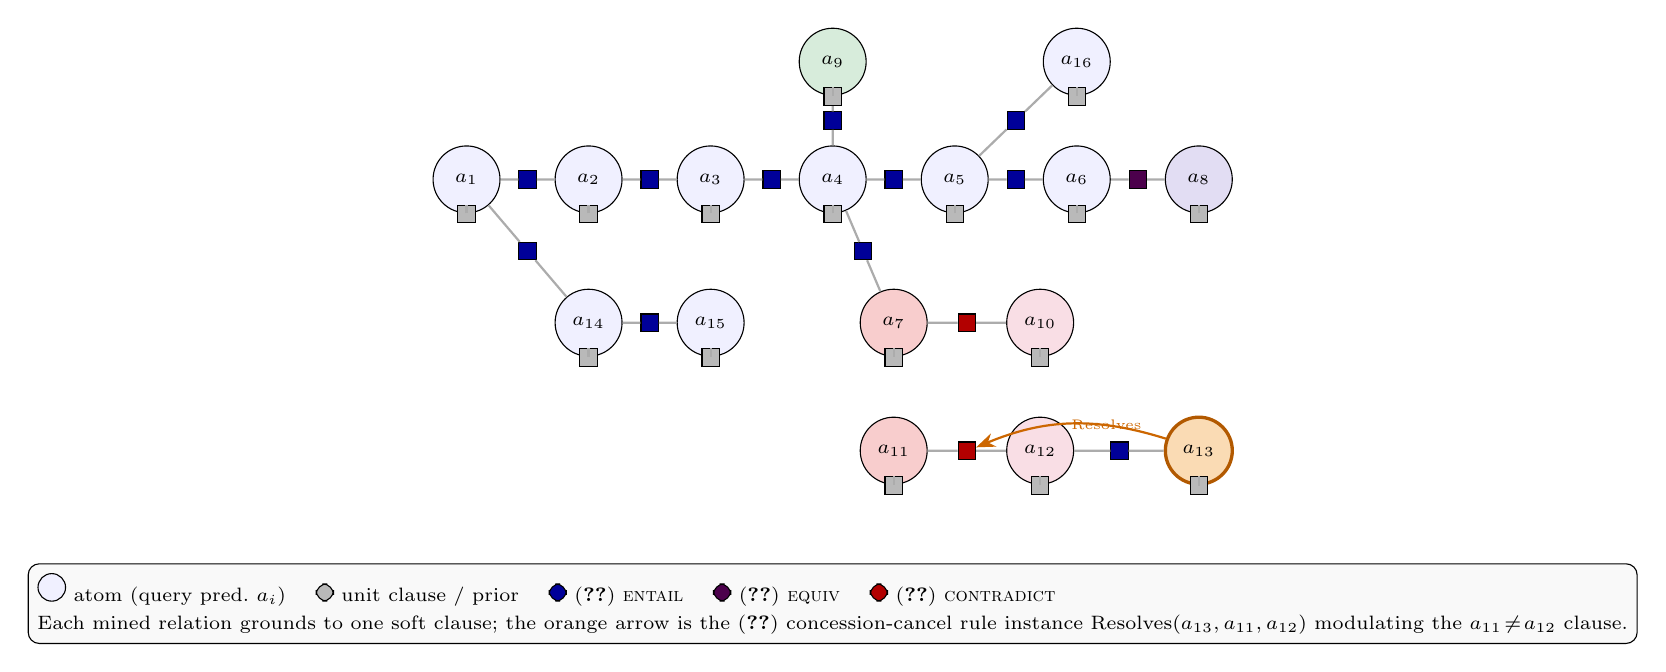
\begin{tikzpicture}[x=15.5mm,y=13mm]
  \node[var]  (a1) at (0,3)   {$a_1$};
  \node[var]  (a2) at (1,3)   {$a_2$};
  \node[var]  (a3) at (2,3)   {$a_3$};
  \node[var]  (a4) at (3,3)   {$a_4$};
  \node[var]  (a5) at (4,3)   {$a_5$};
  \node[var]  (a6) at (5,3)   {$a_6$};
  \node[varQ] (a8) at (6,3)   {$a_8$};
  \node[varE] (a9) at (3,4.15){$a_9$};
  \node[var]  (a16)at (5,4.15){$a_{16}$};
  \node[var]  (a14)at (1,1.6) {$a_{14}$};
  \node[var]  (a15)at (2,1.6) {$a_{15}$};
  \node[varCA](a7) at (3.5,1.6){$a_7$};
  \node[varCB](a10)at (4.7,1.6){$a_{10}$};
  \node[varCA](a11)at (3.5,0.35){$a_{11}$};
  \node[varCB](a12)at (4.7,0.35){$a_{12}$};
  \node[varH] (a13)at (6,0.35) {$a_{13}$};

  \newcommand{\pf}[4]{\node[#1] (#2) at ($(#3)!0.5!(#4)$) {};
    \draw[link] (#3)--(#2); \draw[link] (#2)--(#4);}
  \pf{efac}{f12}{a1}{a2}\pf{efac}{f23}{a2}{a3}\pf{efac}{f34}{a3}{a4}
  \pf{efac}{f45}{a4}{a5}\pf{efac}{f56}{a5}{a6}\pf{qfac}{f68}{a6}{a8}
  \pf{efac}{f94}{a9}{a4}\pf{efac}{f47}{a4}{a7}\pf{efac}{f516}{a5}{a16}
  \pf{efac}{f114}{a1}{a14}\pf{efac}{f1415}{a14}{a15}
  \pf{cfac}{f710}{a7}{a10}\pf{cfac}{f1112}{a11}{a12}\pf{efac}{f1312}{a13}{a12}

  \foreach \v in {a1,a2,a3,a4,a5,a6,a8,a9,a16,a14,a15,a7,a10,a11,a12,a13}{
    \node[ufac] (u\v) at ($(\v)+(0,-0.34)$) {};
    \draw[link] (\v)--(u\v);
  }
  % the resolving-holding rule instance (a13 cancels the a11!=a12 penalty)
  \draw[->,orange!80!black,thick] (a13) to[bend right=20]
     node[right,font=\tiny,pos=0.55]{$\mathrm{Resolves}$} (f1112);

  \node[draw,fill=gray!5,rounded corners,anchor=north,align=left,
        font=\scriptsize] at (3,-0.75) {
    \tikz\node[var,minimum size=3.5mm]{};~atom (query pred.\ $a_i$) \quad
    \tikz\node[ufac]{};~unit clause / prior \quad
    \tikz\node[efac]{};~\eqref{eq:rE} \Ent{} \quad
    \tikz\node[qfac]{};~\eqref{eq:rQ} \Equ{} \quad
    \tikz\node[cfac]{};~\eqref{eq:rC} \Con{}\\[2pt]
    Each mined relation grounds to one soft clause; the orange arrow is the
    \eqref{eq:rR} concession-cancel rule instance $\mathrm{Resolves}(a_{13},a_{11},a_{12})$
    modulating the $a_{11}\!\neq\!a_{12}$ clause.};
\end{tikzpicture}
\caption{The ground Markov network of the AeroParts MLN (pairwise fragment). It has the same
atom variables and one soft clause per relation as the MRF factor graph of the companion
document; the added orange arrow is the one genuinely first-order rule active here ---
$\mathrm{Resolves}(a_{13},a_{11},a_{12})$ --- which cancels the concession penalty
(\S\ref{sec:concession}).}
\label{fig:ground}
\end{figure}

% =====================================================================================
\section{The weight--to--probability mapping}
\label{sec:weights}

This is the technical crux --- what the MRF sidesteps by writing $p$ directly into a factor
table, the MLN must obtain as a log-space weight $w$. We derive it from first principles by
demanding that the pairwise MLN reproduce the with-priors MRF conditional behaviour.

\subsection{Derivation from the per-pair conditional}
Consider one \Ent{} relation $s\!\to\!t$ in isolation, uniform atom priors $\pi{=}0.5$. The
with-priors MRF factor (row-major over $(a_s,a_t)$) is
$\psi=[\,1{-}\pi,\ \pi,\ 1{-}p,\ p\,]=[\,0.5,\,0.5,\,1{-}p,\,p\,]$, which encodes the two
conditionals
\begin{equation}
  P(a_t{=}1\mid a_s{=}0)=\tfrac{0.5}{0.5+0.5}=0.5,
  \qquad
  P(a_t{=}1\mid a_s{=}1)=\tfrac{p}{(1-p)+p}=p .
  \label{eq:cond}
\end{equation}
Now write the MLN implication clause \eqref{eq:rE} with a weight $w$ (and, for a moment, a
target unit clause of weight $w_t$). The clause $a_s\Rightarrow a_t$ is true except at
$(a_s,a_t)=(1,0)$, so the ground potential is
$\exp(w_t\,a_t)\cdot\exp\!\big(w\cdot\mathbb 1[\neg(a_s{=}1\wedge a_t{=}0)]\big)$. Its two
conditionals are
\[
  P(a_t{=}1\mid a_s{=}0)=\sigma(w_t),
  \qquad
  P(a_t{=}1\mid a_s{=}1)=\sigma(w_t+w),
\]
with $\sigma$ the logistic. Matching \eqref{eq:cond} gives $\sigma(w_t)=0.5\Rightarrow w_t=0$
and $\sigma(w)=p$, i.e.
\begin{equation}
  \boxed{\ \ w \;=\; \operatorname{logit}(p)\;=\;\ln\frac{p}{1-p}\ \ }
  \label{eq:wmap}
\end{equation}
For a \Con{} clause $a_s\Rightarrow\neg a_t$ (true except at $(1,1)$) the same argument with
target-false gives $P(a_t{=}1\mid a_s{=}1)=1-p$, again matching the MRF \Con{} row
$[\,p,\,1{-}p\,]$ under $w=\operatorname{logit}(p)$. Numerically (brute force, single edge):
$p{=}0.90\Rightarrow w{=}2.197$ recovers $P(a_t{=}1|a_s{=}1)=0.900$; $p{=}0.93$ contradiction
$\Rightarrow w{=}2.587$ recovers $0.070$; $p{=}0.55\Rightarrow w{=}0.201$ recovers $0.45$.
The mapping is exact, monotone, and calibration-friendly: a \emph{temperature scale} on $p$
becomes an affine scale on $w$.

\subsection{Weights for every AeroParts relation}
Table~\ref{tab:weights} applies \eqref{eq:wmap} to all $14$ mined relations. These are the
per-clause weights of the ground network of Figure~\ref{fig:ground}; they need \emph{no
learning} --- the calibrated $p$ from the miner determines them.

\begin{table}[h]\centering\small
\renewcommand{\arraystretch}{1.12}
\begin{tabular}{@{}llccr@{}}
\toprule
\textbf{Relation} & \textbf{Level-2 sense} & \textbf{coupling} & \textbf{$p$} & \textbf{$w=\operatorname{logit}(p)$}\\
\midrule
$a_1\!\to\!a_2$      & Cause-Effect       & \Ent{} & $.90$ & $2.197$\\
$a_2\!\to\!a_3$      & Cause-Effect       & \Ent{} & $.85$ & $1.735$\\
$a_3\!\to\!a_4$      & Cause-Effect       & \Ent{} & $.70$ & $0.847$\\
$a_4\!\to\!a_5$      & Cause-Effect       & \Ent{} & $.80$ & $1.386$\\
$a_5\!\to\!a_6$      & Cause-Effect       & \Ent{} & $.75$ & $1.099$\\
$a_4\!\to\!a_7$      & Cause-Effect       & \Ent{} & $.65$ & $0.619$\\
$a_9\!\to\!a_4$      & Evidence           & \Ent{} & $.72$ & $0.944$\\
$a_6\!\leftrightarrow\!a_8$ & Restatement & \Equ{} & $.88$ & $1.992$\\
$a_1\!\to\!a_{14}$   & Evidence/Cause     & \Ent{} & $.78$ & $1.266$\\
$a_{14}\!\to\!a_{15}$& Cause-Effect       & \Ent{} & $.70$ & $0.847$\\
$a_5\!\to\!a_{16}$   & Cause-Effect (weak)& \Ent{} & $.60$ & $0.405$\\
$a_{13}\!\to\!a_{12}$& Evidence           & \Ent{} & $.85$ & $1.735$\\
$\mathbf{a_7\!\neq\!a_{10}}$ & \textbf{Contrast (unresolved)} & \Con{} & $\mathbf{.93}$ & $\mathbf{2.587}$\\
$\mathbf{a_{11}\!\neq\!a_{12}}$ & \textbf{Concession (resolved)} & \Con{} & $.80\!\to\!.55$ & $1.386\!\to\!0.201$\\
\bottomrule
\end{tabular}
\caption{Per-clause MLN weights for AeroParts under $w=\operatorname{logit}(p)$
(Eq.~\ref{eq:wmap}). The concession clause's weight is the discounted one when the holding
$a_{13}$ fires the cancel rule (\S\ref{sec:concession}). A confident contradiction carries
the largest weight ($2.587$); a weak causal step the smallest ($0.405$). We keep the two
conflicts as \Con{} here so the exact MLN\,$=$\,MRF equivalence of \S\ref{sec:equiv} is stated
on the same footing as the companion \texttt{coherence\_mrf\_deepdive}; \S\ref{sec:couplings}
shows both are better modeled as \textsc{exclusive} (exactly-one), which is the form the MRF
deep dive adopts for its headline numbers.}
\label{tab:weights}
\end{table}

% =====================================================================================
\section{The AeroParts MLN as an Alchemy program}
\label{sec:alchemy}

We now write the AeroParts model as a concrete \textbf{Alchemy} \citep{mln,alchemy} program:
an \texttt{.mln} file (types, predicate declarations, and weighted formulas) and a companion
\texttt{.db} evidence file (the mined relation graph as ground atoms). This is the executable
form of everything above --- the rule schema of \S\ref{sec:schema} with the weights of
Table~\ref{tab:weights} filled in --- and it runs unchanged under
\texttt{infer -i aeroparts.mln -e aeroparts.db -q Holds} (marginals, MC-SAT) or
\texttt{infer -a} (MAP).

\paragraph{Alchemy syntax, briefly.} A type is declared by listing its constants,
\lstinline[style=mln]!atom = {A1, ..., A16}!; predicates are \lstinline[style=mln]!Capitalised(typed, args)!;
identifiers starting lowercase are \emph{variables} (implicitly universally quantified),
capitalised ones are \emph{constants}. Operators are \verb!!! (not), \verb!^! (and),
\verb!v! (or), \verb!=>! (implies), \verb!<=>! (iff), and \verb!Exist!. A line
``\emph{weight formula}'' is a \emph{soft} formula; a formula ended with a period ``\,.\,''
and no weight is a \emph{hard} constraint. A unit clause of weight $w$ yields marginal
$1/(1+e^{-w})$ --- i.e.\ $w=\operatorname{logit}(p)$, exactly the mapping of
\S\ref{sec:weights}.

\subsection{Declarations and the rule schema (templates)}
The declarations and the universally-quantified \emph{rule templates}
(\S\ref{sec:schema}); these carry a single shared weight per coupling and are what one would
\emph{learn} weights for on a training corpus. \texttt{Holds} is the query (open-world)
predicate; the relation predicates are evidence (closed-world).

\begin{lstlisting}[style=mln]
// ===== aeroparts-templates.mln : types & predicate declarations =====
atom = {A1,A2,A3,A4,A5,A6,A7,A8,A9,A10,A11,A12,A13,A14,A15,A16}

Holds(atom)                 // query predicate: does the claim hold?
Entail(atom,atom)           // evidence: mined inferential couplings
Contradict(atom,atom)
Equiv(atom,atom)
Resolves(atom,atom,atom)    // evidence: holding h adjudicates (i,j)

// ===== rule templates (shared weight per coupling; free vars are  =====
// ===== universally quantified). Learn these weights on a corpus.  =====
w_e  Entail(i,j) ^ Holds(i) => Holds(j)
w_c  Contradict(i,j) ^ Holds(i) => !Holds(j)
w_q  Equiv(i,j) => (Holds(i) <=> Holds(j))

// beyond pairwise (Sec. 6): transitivity, concession-cancel, n-ary conflict
w_t  Entail(i,j) ^ Entail(j,k) => Entail(i,k)
w_r  Resolves(h,i,j) ^ Holds(h) ^ Contradict(i,j) => (Holds(i) <=> Holds(j))
w_d  Contradict(i,j) ^ Contradict(k,j) ^ Holds(i) ^ Holds(k) => !Holds(j)
\end{lstlisting}

\noindent The concession-cancel rule \lstinline[style=mln]!w_r! is the Alchemy rendering of
\eqref{eq:rR}: when a believed holding $h$ resolves the tension $(i,j)$, it \emph{adds}
positive weight to the two endpoints \emph{agreeing} ($\mathrm{Holds}(i)\Leftrightarrow
\mathrm{Holds}(j)$), which counteracts the \lstinline[style=mln]!w_c! penalty that pushes
them apart --- a net cancel whose strength is $w_r$ (hard cancel as $w_r\!\to\!\infty$,
recovering the MRF soft discount at finite $w_r$).

\subsection{The grounded AeroParts model (per-edge weights)}
To pin each mined edge to its own $p$ (rather than a shared learned weight), we ground the
templates: replace the variables by the constants of the actual relation and attach
$w=\operatorname{logit}(p)$ from Table~\ref{tab:weights}. This is the concrete, runnable
AeroParts MLN --- one weighted ground formula per mined relation.

\begin{lstlisting}[style=mln]
// ===== aeroparts.mln : grounded soft formulas (w = logit(p)) =====
// --- entailment / prerequisite / evidence backbone (a_s => a_t) ---
2.197  Holds(A1)  => Holds(A2)      // Cause-Effect p=.90
1.735  Holds(A2)  => Holds(A3)      // Cause-Effect p=.85
0.847  Holds(A3)  => Holds(A4)      // Cause-Effect p=.70
1.386  Holds(A4)  => Holds(A5)      // Cause-Effect p=.80
1.099  Holds(A5)  => Holds(A6)      // Cause-Effect p=.75
0.619  Holds(A4)  => Holds(A7)      // Cause-Effect p=.65
0.944  Holds(A9)  => Holds(A4)      // Evidence     p=.72
1.266  Holds(A1)  => Holds(A14)     // Evidence     p=.78
0.847  Holds(A14) => Holds(A15)     // Cause-Effect p=.70
0.405  Holds(A5)  => Holds(A16)     // Cause-Effect p=.60 (weak)
1.735  Holds(A13) => Holds(A12)     // Evidence     p=.85

// --- equivalence / restatement (a_s <=> a_t) ---
1.992  Holds(A6) <=> Holds(A8)      // Restatement  p=.88

// --- contradictions (a_s => !a_t) ---
2.587  Holds(A7)  => !Holds(A10)    // Contrast, UNRESOLVED  p=.93
1.386  Holds(A11) => !Holds(A12)    // Concession (raw)      p=.80
\end{lstlisting}

\noindent With the holding $a_{13}$ believed, the concession-cancel rule fires on
$(a_{11},a_{12})$ and discounts that last clause; its effective weight drops
$1.386\!\to\!0.201$ ($p:0.80\!\to\!0.55$), i.e.\ in Alchemy one either keeps the raw clause
plus the \lstinline[style=mln]!w_r! rule above, or (equivalently for scoring) replaces the
line with the discounted \lstinline[style=mln]!0.201 Holds(A11) => !Holds(A12)!.

\paragraph{Runnable exact-MRF variant.} The single-implication clauses above are the
\emph{readable} model, but --- as \S\ref{sec:equiv} shows --- they are \emph{coarser} than
the with-priors MRF. To reproduce the MRF numbers exactly, emit instead the
\emph{three-clause} expansion of \S\ref{sec:equiv} per relation, e.g.\ for $a_1\!\to\!a_2$
(\Ent{}, $p{=}.90$): a source unit clause, a (zero-weight, hence omitted) target unit clause,
and the conjunction clause
\begin{lstlisting}[style=mln]
-1.609  Holds(A1)              // source unit:  b = ln((1-p)/0.5)
 2.197  Holds(A1) ^ Holds(A2)  // conjunction:  d = logit(p)
\end{lstlisting}
The templates are the same three per coupling with $(b,c,d)$ from the closed-form table of
\S\ref{sec:equiv}.

\subsection{Evidence: the mined relation graph as a \texttt{.db} file}
The relation predicates are supplied as ground evidence atoms. All other groundings are
closed-world false (e.g.\ no \lstinline[style=mln]!Entail! not listed holds), so only the $14$
mined relations plus the one resolves-fact appear:

\begin{lstlisting}[style=mln]
// ===== aeroparts.db : evidence (the mined relation graph) =====
Entail(A1,A2)    Entail(A2,A3)    Entail(A3,A4)    Entail(A4,A5)
Entail(A5,A6)    Entail(A4,A7)    Entail(A9,A4)    Entail(A1,A14)
Entail(A14,A15)  Entail(A5,A16)   Entail(A13,A12)
Equiv(A6,A8)
Contradict(A7,A10)
Contradict(A11,A12)
Resolves(A13,A11,A12)            // a13 adjudicates the blame tension
\end{lstlisting}

\noindent Querying \lstinline[style=mln]!Holds! returns the per-atom marginals
($q_7{=}0.611$, $q_{10}{=}0.237$, \dots; \S\ref{sec:infer}) under the exact-MRF variant; the
MAP query (\texttt{infer -a}) returns the ``best reading'' $\mathbf a^\star$
(backbone true, $a_7{=}1,a_{10}{=}0$, $a_{12}{=}1,a_{11}{=}0$).

% =====================================================================================
\section{Exact MLN $=$ MRF: the three-clause encoding (and an honest caveat)}
\label{sec:equiv}

A tempting claim is ``the pairwise MLN with $w=\operatorname{logit}(p)$ \emph{is} the
with-priors MRF.'' The per-pair conditional derivation of \S\ref{sec:weights} matched a
\emph{single} edge, but on the full network this is \textbf{false} for the naive
single-implication encoding, and the discrepancy is instructive.

\subsection{Why the single-implication MLN differs}
The MRF's with-priors table is \emph{row-stochastic}: each source-state row sums to $1$
($[0.5,0.5]$ for $a_s{=}0$; $[1{-}p,p]$ for $a_s{=}1$). The single-clause MLN factor
$[e^{w},e^{w},1,e^{w}]$ is \emph{not} --- it rewards the vacuous $a_s{=}0$ rows with $e^w$ on
\emph{both} target states, which inflates the source atom's own marginal relative to the MRF.
Brute force over all $2^{16}$ worlds makes the gap concrete: the single-implication MLN gives
mean marginal support $0.455$ against the MRF's $0.587$, with per-atom marginals differing by
up to $0.31$. \textbf{They are genuinely different models}, not two encodings of one.

Worse, MAP inference of the single-implication MLN is \emph{degenerate}: setting every atom
\emph{false} satisfies every $a_s\Rightarrow a_t$ and every $a_s\Rightarrow\neg a_t$
vacuously (and every $a_s\Leftrightarrow a_t$ as $0{=}0$), so the all-false world violates
\emph{nothing} and the ``most coherent reading'' is the empty one. The implication clauses
must be anchored by evidence (pin the premises) or by unit clauses (below), or the readouts
are meaningless.

\subsection{The fix: expand each factor into three weighted clauses}
Any positive $2\times2$ potential $\psi(a_s,a_t)$ has an exact log-linear form
\begin{equation}
  \ln\psi(a_s,a_t)\;=\;a + b\,a_s + c\,a_t + d\,a_s a_t ,
  \label{eq:loglin}
\end{equation}
i.e.\ a constant, a \emph{source unit clause} ($a_s$, weight $b$), a \emph{target unit
clause} ($a_t$, weight $c$), and a \emph{conjunction clause} ($a_s\wedge a_t$, weight $d$).
Solving \eqref{eq:loglin} against the with-priors tables ($\pi_s{=}0.5$) gives clean closed
forms:
\begin{center}\small
\renewcommand{\arraystretch}{1.25}
\begin{tabular}{@{}lccc@{}}
\toprule
$\tau$ & $b$ (unit $a_s$) & $c$ (unit $a_t$) & $d$ (conj.\ $a_s\wedge a_t$)\\
\midrule
\Ent{}  & $\ln\frac{1-p}{0.5}$ & $0$ & $\operatorname{logit}(p)$\\
\Con{}  & $\ln\frac{p}{0.5}$   & $0$ & $-\operatorname{logit}(p)$\\
\Equ{}  & $\ln\frac{1-p}{p}$   & $\ln\frac{1-p}{p}$ & $2\operatorname{logit}(p)$\\
\bottomrule
\end{tabular}
\end{center}
The conjunction weight is exactly $\pm\operatorname{logit}(p)$ (the ``interaction'' the
implication was meant to carry); the source unit clause is the correction that restores
row-stochasticity. \textbf{With these three clauses per relation, the ground MLN reproduces
the with-priors MRF exactly}: brute force gives mean marginal support $0.5866$ and
$\log Z=-9.751$ for \emph{both}, with zero per-atom difference (to machine precision).
This is the concrete sense in which ``the MLN is a strict generalization of the MRF'': the
pairwise fragment, log-linearly expanded, \emph{is} the MRF; the higher-arity rules of
\S\ref{sec:beyond} are then pure additions on top.

\paragraph{Practical reading.} Adopt the MLN in two stages. \emph{Stage 0} (drop-in): use the
three-clause expansion --- you get the MRF back exactly, still solvable by the shipped WMB
path, and you have paid nothing. \emph{Stage 1} (the reason to be here): add rules
\eqref{eq:rT}--\eqref{eq:rD}, which introduce ground clauses of arity $\ge 3$ and take the
model strictly beyond what any pairwise factorization can represent.

% =====================================================================================
\section{The rules that go beyond pairwise}
\label{sec:beyond}

\subsection{Transitivity of entailment}
Rule \eqref{eq:rT}, $\mathrm{Entail}(i,j)\wedge\mathrm{Entail}(j,k)\Rightarrow\mathrm{Entail}(i,k)$,
lets a two-hop chain contribute \emph{joint} evidence that a pairwise model treats as two
independent links. On AeroParts the chain $a_3\!\to\!a_4\!\to\!a_7$ (both \Ent{}) means
$a_3$ should lend support to $a_7$ even though no $a_3\!\to\!a_7$ relation was mined; the
transitivity rule supplies exactly that ground clause. Two design choices: (i) treat the
\emph{head} $\mathrm{Entail}(i,k)$ as a query predicate (the rule \emph{induces} new
relations, and the induced edge then acts through \eqref{eq:rE}); or (ii) collapse to a
direct soft clause $a_i\wedge\mathrm{path}(i,k)\Rightarrow a_k$. Either way the ground clause
spans three atoms --- not expressible as a product of pairwise factors. The weight $w_t$
governs how much a mined chain is allowed to ``complete''; it is the one weight here that
genuinely wants \emph{learning} (from held-out coherence judgements) rather than a closed
form, because it is not tied to a single mined $p$.

\subsection{Concession cancels the contradiction penalty}
\label{sec:concession}
This is the headline capability. A Concession (``although $X$, still $Y$'') or an adjudicating
\emph{holding} is not a coherence defect --- it is a contradiction the text \emph{itself
resolves}. The MRF can only approximate this by hand-softening the contradiction strength
(the $0.80\!\to\!0.55$ discount of the companion document). The MLN expresses it directly,
rule \eqref{eq:rR}:
\[
   w_r:\quad \mathrm{Resolves}(h,i,j)\ \wedge\ a_h\ \Rightarrow\ \neg\,\mathrm{Penalize}(i,j),
\]
which, when the holding $a_h$ holds, \emph{removes} (or, with finite $w_r$, discounts) the
ground $a_i\!\neq\!a_j$ contradiction clause rather than merely lowering its $p$. On
AeroParts, $\mathrm{Resolves}(a_{13},a_{11},a_{12})$ fires because the ``pilots not at fault''
holding $a_{13}$ is believed, cancelling the $a_{11}\!\neq\!a_{12}$ blame contradiction while
leaving the \emph{unresolved} casualty contradiction $a_7\!\neq\!a_{10}$ untouched. The effect
on the score is exactly the concession row of Table~\ref{tab:menu}: mean support rises
$0.587\!\to\!0.601$, and it does so \emph{because a rule fired}, not because a human retuned a
number. With a \emph{hard} cancel ($w_r\!\to\!\infty$) the clause vanishes entirely; with a
finite $w_r$ tied to $\pi_h$ it recovers the MRF's soft discount $p_{\text{eff}}=p(1-\lambda\pi_h)$
as a special case --- so the MRF's concession handling is the $w_r$-finite projection of this
rule.

\subsection{$n$-ary ``doubly-contradicted'' penalty}
Rule \eqref{eq:rD} says an atom contradicted by \emph{two} independent asserted atoms should
be penalized harder than the sum of two pairwise penalties would suggest. This is a $3$-atom
(or higher) ground clause with a super-additive weight --- the kind of ``two independent
sources disagree with you'' reasoning that a pairwise model, which factorizes over pairs,
structurally cannot represent. It is optional on AeroParts (no atom is doubly contradicted)
but is the template for real multi-source disagreement.

% =====================================================================================
\section{Learning the rule weights}
\label{sec:learn}

The pairwise weights are a closed form of the mined $p$ ($w=\operatorname{logit}(p)$,
\S\ref{sec:weights}) and need \emph{no} learning. The \emph{beyond-pairwise} rule weights
$w_t$ (transitivity), $w_r$ (concession-cancel), $w_d$ (double-conflict) are \textbf{not}
tied to any single mined relation --- they express how much such structural patterns should
count --- and must be \emph{learned} from data. This section shows the training corpus that
does it, in Alchemy's \texttt{learnwts} format.

\subsection{What supervision is available}
The learning signal is a set of responses whose atom truths are \emph{known}. Two sources
give it cheaply, without new annotation:
\begin{itemize}[leftmargin=*,nosep]
  \item \textbf{The five ideation examples} (\texttt{example-1..5}) and AeroParts, each
        hand-annotated with which atoms hold in the ``correct reading'' (the coherent atoms
        true; the retracted/losing side of each contradiction false). These become the
        ground-truth \texttt{Holds} atoms.
  \item \textbf{Coherent/incoherent minimal pairs}: for each response, the base version and a
        \emph{corrupted} version (inject a spurious contradiction, drop a resolving holding, or
        scramble order --- the \emph{Renda} S-vs-K manipulation). The pair teaches the weights
        to \emph{separate} coherent from incoherent, which a single polarity cannot.
\end{itemize}
Each labeled response is one \emph{training database} (\texttt{.db}): the evidence relation
graph (as in \S\ref{sec:alchemy}) \emph{plus} the observed truth of every \texttt{Holds}
atom. \texttt{Holds} is the non-evidence (query) predicate we learn to predict; the relation
predicates stay evidence.

\subsection{A training database (one labeled response)}
The AeroParts training database augments the evidence \texttt{.db} of \S\ref{sec:alchemy}
with the gold \texttt{Holds} atoms of its coherent reading. Closed-world: any \texttt{Holds}
\emph{not} listed is observed false --- so the retracted blame $a_{11}$ and the false-casualty
claim $a_{10}$ are absent by omission (or written negated for emphasis).

\begin{lstlisting}[style=mln]
// ===== aeroparts-train.db : evidence + gold atom truths =====
// --- evidence: the mined relation graph (as in aeroparts.db) ---
Entail(A1,A2)    Entail(A2,A3)    Entail(A3,A4)    Entail(A4,A5)
Entail(A5,A6)    Entail(A4,A7)    Entail(A9,A4)    Entail(A1,A14)
Entail(A14,A15)  Entail(A5,A16)   Entail(A13,A12)
Equiv(A6,A8)     Contradict(A7,A10)   Contradict(A11,A12)
Resolves(A13,A11,A12)

// --- gold: which atoms hold in the correct reading ---
Holds(A1)  Holds(A2)  Holds(A3)  Holds(A4)  Holds(A5)  Holds(A6)
Holds(A7)             Holds(A8)  Holds(A9)
Holds(A12) Holds(A13) Holds(A14) Holds(A15) Holds(A16)
// omitted (closed-world false): Holds(A10), Holds(A11) -- the losing/retracted sides
!Holds(A10)   // wire-report casualty claim: rejected
!Holds(A11)   // pilot-error blame: retracted by the holding a13
\end{lstlisting}

\subsection{The corrupted twin (the negative of the pair)}
The same response with a spurious contradiction injected ($a_3\!\neq\!a_{12}$, the
\emph{worse} variant of the companion MRF deep-dive) --- and \emph{no} resolving holding for
it --- is a second database whose gold reading now cannot satisfy everything. It is what
pushes $w_r$ up (concessions \emph{should} be resolvable) and $w_d$ up (a doubly-attacked
atom \emph{should} fall).

\begin{lstlisting}[style=mln]
// ===== aeroparts-worse-train.db : corrupted twin =====
Entail(A1,A2)   ... (same backbone) ...   Entail(A13,A12)
Equiv(A6,A8)    Contradict(A7,A10)   Contradict(A11,A12)
Contradict(A3,A12)          // INJECTED spurious conflict, unresolved
Resolves(A13,A11,A12)
// gold reading: a12 now doubly contradicted (by a3 and a11) -> a12 falls
Holds(A1) ... Holds(A11)    // (backbone as before)
!Holds(A12)  !Holds(A10)    // the doubly/among-contradicted losers
\end{lstlisting}

\subsection{Running the learner}
Generative weight learning maximizes the (pseudo-)likelihood of the gold \texttt{Holds}
atoms across all training databases; discriminative learning (\texttt{-d}) maximizes the
conditional likelihood of \texttt{Holds} given the relation evidence, which is what we want
(the relations are always observed). Both take the \emph{template} \texttt{.mln} of
\S\ref{sec:alchemy}.1 --- the shared-weight rules, \emph{not} the pre-grounded per-edge file
--- and fit one weight per formula:

\begin{lstlisting}[style=mln]
learnwts -d -i aeroparts-templates.mln -o aeroparts-learned.mln \
         -t aeroparts-train.db,aeroparts-worse-train.db,renda-S.db,renda-K.db,... \
         -ne Holds
\end{lstlisting}

\noindent \texttt{-ne Holds} declares \texttt{Holds} the non-evidence predicate;
\texttt{-t} takes the comma-separated training databases (one per labeled response);
\texttt{aeroparts-learned.mln} contains the fitted $w_e,w_c,w_q,w_t,w_r,w_d$. In practice we
\emph{fix} the pairwise weights at their closed form $\operatorname{logit}(p)$ (they are
already calibrated) and learn \emph{only} the structural $w_t,w_r,w_d$ --- so the corpus need
only be large enough to estimate three numbers, not the whole model. A held-out split of the
same corpus then calibrates the readouts of \S\ref{sec:scoring} (temperature scaling) against
human coherence ratings.

\paragraph{Corpus size and the per-relation-\texttt{+} option.} Three structural weights need
only tens of labeled responses. If instead one wanted a \emph{separate} learned weight per
\emph{discourse sense} (Cause-Effect vs.\ Evidence vs.\ Restatement, rather than one shared
$w_e$), Alchemy's \texttt{+} operator on the sense argument
--- \lstinline[style=mln]!w  Sense(i,j,+s) ^ Holds(i) => Holds(j)! --- makes the learner fit
one weight per sense constant \texttt{s}, at the cost of needing enough examples of each
sense. This is the bridge back to the Level-2 taxonomy: the compile map's strength priors
(companion doc) become \emph{learned} per-sense weights.

% =====================================================================================
\section{Inference}
\label{sec:infer}

\subsection{MAP: the most coherent reading (MaxWalkSAT)}
MAP inference returns the single most probable world
$\mathbf a^\star=\arg\max_{\mathbf a}\sum_k w_k n_k(\mathbf a)$ --- the ``best reading'' of
the response, and the assignment of maximum satisfied weight. On AeroParts, exact MAP over
the three-clause (MRF-equivalent) network sets the \emph{entire causal backbone} true and
resolves \emph{both} contradictions decisively: $a_7{=}1,a_{10}{=}0$ (accept ``no
casualties'', reject ``three died'') and $a_{12}{=}1,a_{11}{=}0$ (keep the adjudicated defect
finding, reject the retracted pilot-error blame). Its log-mass is $\log\mathrm{mass}(\mathbf
a^\star)=-15.16$ and \emph{zero} relations are violated at $\mathbf a^\star$ --- a
contradiction is ``resolved'' at MAP simply by taking one side. In production, exact MAP is
NP-hard; MaxWalkSAT \citep{mln} is the standard stochastic-local-search solver.

\subsection{Marginals: per-atom support (MC-SAT)}
Marginal inference returns $q_i=P(a_i{=}1)$, the per-atom analogue of the MRF marginals.
Because the three-clause network equals the MRF, the exact marginals coincide:
$q_7{=}0.611$, $q_{10}{=}0.237$ (the casualty loser driven down), $q_{11}{=}0.441$,
$q_{12}{=}0.528$, backbone $a_2$--$a_6$ at $0.68$--$0.76$, mean $0.587$. Exact marginals /
$\log Z$ are \#P-hard for a general MLN; the standard sampler is MC-SAT \citep{mln}, with
lifted belief propagation an option when the rules have symmetry. For the pairwise fragment
we can bypass all of this and use the shipped Merlin WMB path directly on the equivalent MRF
(\S\ref{sec:equiv}); MC-SAT is needed only once the higher-arity rules
(\S\ref{sec:beyond}) are switched on.

% =====================================================================================
\section{Scoring the coherence of the whole response}
\label{sec:scoring}

Per the design decision for this document, we present the \emph{menu} of readouts
even-handedly rather than crowning a single headline, and recommend reporting a small
\textbf{vector}. All four are functionals of the same ground MLN; they answer subtly
different questions and, as the concession column shows, they do not always agree.

\paragraph{M1 --- Mean marginal support (belief).}
$\mathrm{LCS}_{\text{M1}}=\frac1n\sum_i q_i$, the MLN's per-atom belief averaged. Monotone
in coherence, in $[0,1]$, no free constant, and directly comparable to the MRF and to
FactReasoner's own precision-style aggregate. On AeroParts it runs
$0.587\to0.601\to0.620$ across base $\to$ concession-resolved $\to$ coherent (Table~\ref{tab:menu}).

\paragraph{M2 --- MAP violated-weight energy (the MLN-native readout).}
The quantity MLN inference most naturally produces: the total weight of the clauses the best
world must \emph{violate},
\[
   \mathcal V(\mathbf a^\star)=\sum_k w_k\,\big(N_k-n_k(\mathbf a^\star)\big),
   \qquad
   \mathrm{LCS}_{\text{M2}}=\sigma\!\big(-\mathcal V(\mathbf a^\star)/T\big),
\]
squashed to $[0,1]$ with a temperature $T$. It says ``how much did the most coherent reading
still have to break?'' On AeroParts the MRF-equivalent MAP violates \emph{zero} weight
(both contradictions are resolved by taking a side), so $\mathcal V{=}0$ --- which exposes
M2's weakness: it scores the \emph{best-case} reading, and a single MAP world can always
sidestep a contradiction by choosing one endpoint. It is most useful when premises are pinned
as evidence (then the MAP must confront the contradiction) or with the double-conflict rule
\eqref{eq:rD} that no single assignment can satisfy.

\paragraph{M3 --- Reified coherence node $P(R{=}1)$.}
Add one binary $R$ with a rule ``$R\Rightarrow(\text{every relation satisfied})$'', i.e.\ a
noisy-\textsc{and}: $R{=}1$ pays a factor $1-p_r$ for every relation the world breaks. Reported as
$P(R{=}1)$ this is a single interpretable $[0,1]$ probability. It folds in \emph{all}
relation types but introduces a prior $\rho$ (a tuned constant) and, like M2, reads
whether \emph{the conflict is active} --- so it \emph{dips} at the concession variant
(Table~\ref{tab:menu}, non-monotone), the shared quirk analysed in the MRF deep-dive.

\paragraph{M4 --- Normalized log-partition (structural satisfiability).}
$\mathrm{LCS}_{\text{M4}}=(\log Z-\log Z_{\min})/(\log Z_{\max}-\log Z_{\min})$, with
$Z_{\max}$ the contradiction-free network (upper reference) and $Z_{\min}$ the MAP-world
mass (a provable lower bound, since $Z$ is a sum of non-negative terms). $\log Z$ is the
total mass the weighted rules retain; a confident contradiction costs $\approx$~a full nat.
Monotone and the most contradiction-sensitive readout, but a whole-network quantity with no
per-atom attribution, and it needs the two reference runs. On the AeroParts base network,
$\log Z=-9.75$, $\ \log Z_{\min}=-15.16$, and $\ \log Z_{\max}=-8.25$, giving M4~$=0.78$.

\begin{table}[h]\centering\small
\renewcommand{\arraystretch}{1.15}
\begin{tabular}{@{}lcccc@{}}
\toprule
\textbf{Variant} & M1 mean supp. & M2 MAP viol.\ $\mathcal V$ & M3 $P(R{=}1)$ & M4 $\log Z$ (norm.)\\
\midrule
base                    & $0.587$ & $0.00$ & $0.150$ & $-9.75\ (0.78)$\\
concession-resolved     & $0.601$ & $0.00$ & $\mathbf{0.146}$ & $-9.66\ (0.80)$\\
coherent (no contra.)   & $0.620$ & $0.00$ & $0.181$ & $-8.25\ (1.00)$\\
\midrule
\textbf{monotone?}      & \textbf{yes} & degenerate & no (bold) & \textbf{yes}\\
\bottomrule
\end{tabular}
\caption{The four MLN readouts across the coherence-ordered family (exact, $2^{16}$ worlds;
three-clause MRF-equivalent network). M1 and M4 are monotone; M3 inherits the concession
non-monotonicity (bold, cf.\ MRF deep-dive \S9); M2's MAP energy is degenerate here because a
single best world resolves both contradictions by taking a side. \textbf{Recommendation:}
report the vector $(\text{M1},\ \log Z,\ \text{M2 when premises are pinned})$; use M3 only as
an interpretable companion.}
\label{tab:menu}
\end{table}

\paragraph{Recommendation (no single headline).} Report a \textbf{small vector}: M1 (belief,
comparable across models and to the MRF), raw $\log Z$ / M4 (contradiction sensitivity), and
M2 \emph{only} when the analysis pins premises as evidence so the MAP must actually confront
the conflicts. Keep M3 as an optional interpretable read-out. The reasoning is the same
lesson as the MRF deep-dive --- a belief-based score (M1, M4) tracks coherence monotonically,
whereas an ``is-the-conflict-active'' score (M2, M3) can move the wrong way when a resolved
tension is softened.

% =====================================================================================
\section{Algorithm}
\label{sec:algo}

\begin{figure}[h]\centering
\fbox{\parbox{0.94\textwidth}{\small
\textbf{Algorithm 1: \textsc{ComputeLCS-MLN}$(y)$}\\[2pt]
\textbf{Input:} response $y$; miner $\mathcal M$; rule weights $\{w_t,w_r,w_d\}$; prior $\pi$.\\
\textbf{Output:} coherence vector $(\text{M1},\ \log Z,\ \text{M2},\ \text{M3})$, marginals $\{q_i\}$.
\begin{enumerate}[leftmargin=1.4em,nosep,label=\arabic*.]
  \item $A\leftarrow\textsc{AtomizeAndDecontextualize}(y)$;\ \ $C\leftarrow\textsc{CandidatePairs}(A)$
        \hfill// as MRF (order-window $+$ similarity prune)
  \item \textbf{for each} $(a_i,a_j)\in C$: $(\text{sense},\tau,p)\leftarrow\mathcal M(a_i,a_j)$;
        set evidence pred.\ $\mathrm{Entail}/\mathrm{Contradict}/\mathrm{Equiv}(i,j)$; drop \None{}.
  \item \textbf{for each} relation: emit the three log-linear clauses of \S\ref{sec:equiv}
        with $b,c,d$ from $p$ \hfill// Stage-0: exact MRF re-encoding
  \item \textbf{if} sense $=$ Concession and $\exists\,h$: assert $\mathrm{Resolves}(h,i,j)$
        \hfill// fires rule \eqref{eq:rR}
  \item ground rules \eqref{eq:rT}--\eqref{eq:rD} (transitivity, concession-cancel, double-conflict)
        \hfill// Stage-1: the beyond-pairwise clauses
  \item \textbf{if} only pairwise clauses present: solve on the equivalent MRF via Merlin WMB\\
        \textbf{else}: MC-SAT for $\{q_i\},\log Z$; MaxWalkSAT for $\mathbf a^\star$
  \item M1 $\leftarrow\frac1n\sum_i q_i$;\ \ M2 $\leftarrow\sigma(-\mathcal V(\mathbf a^\star)/T)$;\ \
        M3 $\leftarrow P(R{=}1)$;\ \ M4 $\leftarrow$ normalized $\log Z$
  \item \textbf{return} the vector, $\{q_i\}$, and $\mathbf a^\star$ (the ``best reading'')
\end{enumerate}
}}
\label{alg:mln}
\end{figure}

\paragraph{Cost.} Steps 1--2 (miner calls) dominate, as in the MRF. Step 6 is where the MLN
diverges: the pairwise fragment is free (reuses WMB); the higher-arity rules require MC-SAT /
MaxWalkSAT (a new dependency, \#P-hard marginals). This is the reuse-vs-expressivity trade to
weigh against the extra rules' value.

% =====================================================================================
\section{MRF vs.\ MLN --- when to use which}
\label{sec:vs}

\begin{center}\small
\renewcommand{\arraystretch}{1.15}
\begin{tabular}{@{}p{3.0cm}p{5.3cm}p{5.3cm}@{}}
\toprule
 & \textbf{MRF (companion doc)} & \textbf{MLN (this doc)}\\
\midrule
Parameters      & $p$ enters a factor table directly; \emph{no learning} & pairwise $w=\operatorname{logit}(p)$ closed-form; \emph{but} rule weights $w_t,w_r,w_d$ learned from a labeled corpus (\S\ref{sec:learn})\\
Concession      & hand-softened $p$ (Eq.~for $p_{\text{eff}}$) & first-class \emph{cancel rule} \eqref{eq:rR}; MRF discount is its finite-$w_r$ projection\\
Beyond pairwise & impossible (pairwise factorization) & transitivity, $n$-ary conflict --- ground clauses of arity $\ge3$\\
Inference       & Merlin WMB, sub-second, shipped & pairwise: reuse WMB; with rules: MC-SAT / MaxWalkSAT (new dep., \#P-hard)\\
Equivalence     & --- & three-clause expansion (\S\ref{sec:equiv}) reproduces the MRF exactly\\
Recommendation  & \textbf{primary} (max reuse) & \textbf{research branch} for rules \emph{over} relations\\
\bottomrule
\end{tabular}
\end{center}

\paragraph{Bottom line.} The MLN is a strict generalization of the MRF: its pairwise
fragment, log-linearly expanded with $w=\operatorname{logit}(p)$, \emph{is} the with-priors
MRF (verified exactly: identical marginals and $\log Z$). Adopt the MRF as the default; reach
for the MLN precisely when the analysis needs rules \emph{over} relations that no pairwise
model can express --- above all the \emph{concession-cancels-penalty} rule, which turns the
MRF's hand-tuned discount into a rule that fires automatically when a resolving holding is
present, and transitivity/double-conflict, which let multi-hop and multi-source structure
speak.

% =====================================================================================
\section{Beyond entail / contradict / equiv: a richer coupling vocabulary}
\label{sec:couplings}

The Level-1 vocabulary so far is $\{\Ent,\Con,\Equ,\None\}$ --- FactReasoner's NLI edge
types. That is a deliberate minimum, not a ceiling. This section explores what \emph{other}
coupling relations are worth adding, taking the two formalisms in turn: first the MLN, whose
first-order rules impose almost no vocabulary limit, then the MRF, whose pairwise factor is
provably a \emph{three-parameter} family --- which both bounds it and, pleasantly, shows
several ``new'' couplings are already reachable.

\subsection{In the MLN: the vocabulary is open}
\label{sec:couplings-mln}
An MLN coupling is just a weighted formula, so ``adding a coupling'' means adding a rule
template plus (for a mineable one) an evidence predicate. There is no 2-atom or fixed-arity
restriction. Candidates that earn their place on the coherence task:

\begin{itemize}[leftmargin=*]
  \item \textbf{Necessary condition / presupposition} $\mathrm{Requires}(i,j)$: $a_i$ can hold
        \emph{only if} $a_j$ does --- ``$a_i$ presupposes $a_j$''. Rule
        \(w:\ \mathrm{Requires}(i,j)\wedge a_i\Rightarrow a_j\), capturing presupposition,
        definite-reference licensing, and ``necessary cause'' (vs.\ \Ent's ``sufficient
        cause''). Directed; pairwise. Note it forbids the same world as \Ent{}, so in the MRF
        it is just entailment with the edge reversed (\S\ref{sec:couplings-mrf}); the MLN
        keeps it as a \emph{named} rule when the interpretability matters.
  \item \textbf{Mutual exclusion among a set} $\mathrm{Alt}(i,j,\dots)$: at most one of a
        \emph{group} of claims may hold (competing hypotheses, incompatible values of one
        slot). For a set $S$, \(w:\ \bigwedge_{i\ne j\in S}\neg(a_i\wedge a_j)\) --- an
        $n$-ary constraint. The two-element case degenerates to \Con{}, but the group case
        (``the report blames exactly one of pilot-error, metallurgy, maintenance'') is
        genuinely $>2$-ary and \textbf{not} pairwise.
  \item \textbf{Defeasible / default} $\mathrm{DefaultTrue}(i)$ with $\mathrm{Except}(e,i)$:
        $a_i$ holds \emph{unless} an exception $a_e$ fires ---
        \(w:\ \mathrm{DefaultTrue}(i)\wedge\neg a_e\Rightarrow a_i\). This is the general form
        of the concession-cancel rule (\S\ref{sec:concession}) and of non-monotonic
        ``holds-by-default-then-retracted'' patterns; it needs the exception atom, so
        arity~$\ge 3$.
  \item \textbf{Corroboration / joint support} $\mathrm{Supports}(i,g),\mathrm{Supports}(j,g)$:
        two independent claims each raise a goal $a_g$, and \emph{jointly} more than the sum
        --- a super-additive $\bigwedge$-rule, the positive-evidence twin of the
        double-conflict rule \eqref{eq:rD}. Multi-source agreement; $n$-ary.
  \item \textbf{Graded / typed entailment via the \texttt{+} operator}: rather than a new
        coupling, split \Ent{} \emph{by discourse sense} ---
        \(w:\ \mathrm{Sense}(i,j,+s)\wedge a_i\Rightarrow a_j\) --- so Cause-Effect, Evidence,
        and Condition each get their own learned weight (\S\ref{sec:learn}). This is the
        cheapest ``richer vocabulary'': same arity, more resolution.
  \item \textbf{Quantified / structural} (transitivity \eqref{eq:rT}, and ``every claim in a
        group entails the conclusion''): first-order rules over the relation predicates
        themselves, unbounded arity. Only the MLN can state these.
\end{itemize}
The price is uniform: each new template adds a weight to learn (\S\ref{sec:learn}) and, if it
grounds to arity $\ge 3$, forces MC-SAT/MaxWalkSAT rather than the shipped WMB path. The MLN
never says ``impossible'' --- it says ``one more rule, one more weight.''

\subsection{In the MRF: the pairwise factor is a closed 3-parameter family}
\label{sec:couplings-mrf}
The MRF confines a coupling to a single $2\times2$ factor over $(a_s,a_t)$. Its log-linear
form (\S\ref{sec:equiv}) is $\ln\psi=a+b\,a_s+c\,a_t+d\,a_s a_t$; after normalization only
\emph{three} numbers are free:
\[
  b\ \text{(source bias)},\qquad c\ \text{(target bias)},\qquad d\ \text{(interaction)}.
\]
\textbf{Every conceivable pairwise coupling is a point in this 3-D space}, so the MRF's entire
coupling vocabulary is characterized once and for all. The cleanest way to enumerate the
useful ones is by \emph{which world(s) the factor penalizes} --- a soft constraint is exactly
a preference against some subset of the four worlds $(a_s,a_t)$. This gives a small, complete
catalogue (Table~\ref{tab:bcd}): \textbf{four} ``forbid one corner'' couplings (one per
world) and \textbf{two} ``forbid a diagonal'' couplings.

\begin{table}[h]\centering\small
\renewcommand{\arraystretch}{1.2}
\begin{tabular}{@{}llp{4.4cm}rrr@{}}
\toprule
\textbf{Penalized world} & \textbf{Coupling} & \textbf{Reading} & $b$ & $c$ & $d$\\
\midrule
$(s{=}1,t{=}0)$ & \Ent{} $s\!\Rightarrow\!t$        & sufficient cond.\ / cause / evidence & $-1.61$ & $0$ & $+2.20$\\
\rowcolor{cRule!40}
$(s{=}0,t{=}1)$ & \textbf{Reverse-entail} $t\!\Rightarrow\!s$ & necessary cond.\ / presupposition / ``$t$ needs $s$'' & $0$ & $-1.61$ & $+2.20$\\
$(s{=}1,t{=}1)$ & \Con{} not-both                   & contrast / mutual exclusion (of two) & $+0.59$ & $0$ & $-2.20$\\
\rowcolor{cRule!40}
$(s{=}0,t{=}0)$ & \textbf{Co-necessity} at-least-one & disjunction / joint prerequisite (``not neither'') & $+1.61$ & $+1.61$ & $-1.02$\\
\midrule
$s\ne t$ (off-diag.) & \Equ{} $s\!\Leftrightarrow\!t$ & restatement / mutual entailment & $-2.20$ & $-2.20$ & $+4.39$\\
\rowcolor{cRule!40}
$s=t$ (diag.)   & \textbf{Exclusive} exactly-one     & alternatives (``exactly one holds'') & $+2.20$ & $+2.20$ & $-4.39$\\
\bottomrule
\end{tabular}
\caption{The \emph{complete} pairwise coupling catalogue, indexed by the world(s) each factor
penalizes ($p{=}0.9$, $\pi_s{=}0.5$). The shipped vocabulary uses only \Ent{}, \Con{}, and
\Equ{} (white); \emph{three} more couplings are already inside the 3-parameter family and cost
only a new table (shaded): \textbf{Reverse-entail} (necessary condition/presupposition),
\textbf{Co-necessity} (``at least one''), and \textbf{Exclusive} (exactly-one/XOR). The sign
of the interaction $d$ sets the character ($d{>}0$ positive/agreement, $d{<}0$
negative/opposition, $d{=}0$ is \None{}); the biases $b,c$ place the direction.}
\label{tab:bcd}
\end{table}

\paragraph{A subtlety worth stating: entailment and ``necessary condition'' are the same
constraint.} It is tempting to add ``$s$ requires $t$'' as a new coupling, but as a
\emph{factor} it penalizes the world $(s{=}1,t{=}0)$ --- \emph{exactly} the world \Ent{}
penalizes. A necessary condition and a sufficient condition forbid the same corner; they
differ only in which atom the analyst calls source and which direction the mined edge points.
The genuinely new corner is $(s{=}0,t{=}1)$ --- \textbf{reverse-entail} $t\!\Rightarrow\!s$
--- which the miner produces simply by emitting the edge the other way. So ``richer
direction'' in the MRF is a mining choice, not a new table.

\paragraph{What the MRF gains for free.} Beyond re-orienting entailment, two couplings with a
\emph{new penalized world} are one table each:
\begin{itemize}[leftmargin=*,nosep]
  \item \textbf{Exclusive} (exactly-one / mutual exclusion of \emph{two} claims): table
        $[\,1{-}p,\,p,\,p,\,1{-}p\,]$ over $(a_s,a_t)$ --- \Equ{} with the interaction sign
        flipped, penalizing \emph{both} same-value worlds, for genuine alternatives (``the
        cause was $X$ or $Y$, not neither and not both'').
  \item \textbf{Co-necessity} (``at least one holds''): table $[\,1{-}p,\,\pi,\,\pi,\,p\,]$
        --- penalizes the both-false world, for a disjunction or a joint prerequisite (``at
        least one of the two supporting findings must hold'').
\end{itemize}

\paragraph{What the MRF provably cannot do.} Anything whose ``penalized world'' is not a
function of a \emph{single} pair leaves the 3-D family and is unrepresentable as one factor:
\emph{mutual exclusion among $>2$ claims}, \emph{defeasible/default} (needs the exception
atom), \emph{joint corroboration} (super-additivity is a 3-clique effect), and all
\emph{quantified/transitive} rules. The escape hatch is the same reification the scoring
section already uses (\S\ref{sec:scoring}, the $R$ node): introduce an \textbf{auxiliary
variable} that ANDs/ORs the group and attach pairwise factors to \emph{it}. E.g.\ ``at most
one of $\{a_i,a_j,a_k\}$'' becomes an auxiliary $U=\bigvee_{\text{pairs}}(a\wedge a')$ with a
unary factor pinning $U{=}0$ --- three pairwise factors plus one aux node, all within the
shipped \texttt{MarkovNetwork}. This recovers the $n$-ary couplings at the cost of extra
variables and the usual loss of a clean per-atom reading; it is exactly the boundary where
one should instead reach for the MLN.

\paragraph{Recommendation.} Extend the \emph{Level-1} vocabulary from three couplings to
\textbf{five} --- add \textbf{Exclusive} (exactly-one) and \textbf{Co-necessity}
(at-least-one) --- in \emph{both} models: they are common in argumentative text (competing
hypotheses; disjunctive support), they are single factor tables in the MRF (drop-in to
\texttt{\_edge\_factor\_values}), and single rule templates in the MLN. Treat necessary
condition / presupposition not as a sixth type but as \textbf{reverse-entail} --- the miner
emits the entailment edge in the other direction. Keep the genuinely higher-arity couplings
(group mutual-exclusion over $>2$ claims, defeasible/default, corroboration, transitivity) as
\textbf{MLN-only} extensions, with the MRF reaching them only through auxiliary-variable
reification when a full MLN is not warranted. The Level-2 discourse senses map onto the
enlarged set with no change to the compile philosophy: a two-way \emph{Disjunction} /
mutually-exclusive \emph{Alternative}~$\to$~\textbf{Exclusive}; a ``at least one of these
grounds must hold'' \emph{Conjunction-of-support}~$\to$~\textbf{Co-necessity};
Precondition/Background~$\to$~\textbf{reverse-entail}.

% =====================================================================================
\section{Summary}
\label{sec:summary}

\begin{itemize}[leftmargin=*]
  \item \textbf{Model:} weighted first-order rules \eqref{eq:rE}--\eqref{eq:rD} over atom
        (query) and relation (evidence) predicates; \emph{grounding} produces a ground Markov
        network with one soft clause per relation plus the higher-arity clauses.
  \item \textbf{Weight mapping:} $w=\operatorname{logit}(p)$ (Eq.~\ref{eq:wmap}), derived from
        the per-pair conditional; closed-form, no learning for the pairwise fragment; the
        full AeroParts weight table is Table~\ref{tab:weights}.
  \item \textbf{Exact equivalence:} the naive single-implication MLN is a \emph{coarser}
        model (mean support $0.455$ vs.\ $0.587$, and a degenerate all-false MAP); the
        \textbf{three-clause log-linear expansion} reproduces the with-priors MRF \emph{exactly}
        (mean $0.5866$, $\log Z=-9.751$ for both).
  \item \textbf{Beyond pairwise:} transitivity of entailment, the
        \emph{concession-cancels-penalty} rule (the MRF discount is its finite-weight
        projection), and $n$-ary double-conflict --- ground clauses no pairwise factorization
        can represent.
  \item \textbf{Learning:} the pairwise weights are closed-form; only the structural
        $w_t,w_r,w_d$ are learned, from a corpus of labeled responses --- each a training
        \texttt{.db} of the mined relation graph \emph{plus} the gold \texttt{Holds} atoms of
        its correct reading, with coherent/corrupted twins as the negatives, fitted by
        \texttt{learnwts -d -ne Holds} (\S\ref{sec:learn}).
  \item \textbf{Scoring:} report a \emph{vector} --- M1 mean marginal support (belief,
        comparable, monotone), $\log Z$ / M4 (contradiction-sensitive), M2 MAP violated-weight
        energy (MLN-native, but best-case and degenerate unless premises are pinned), M3
        reified $P(R{=}1)$ (interpretable companion, non-monotone under concession). No single
        headline.
  \item \textbf{Behaviour:} on AeroParts M1 moves $0.587$ (base) $\to 0.601$ (concession
        \emph{rule} fires) $\to 0.620$ (coherent), coinciding with the MRF by the equivalence.
\end{itemize}

% =====================================================================================
\begin{thebibliography}{9}\small
\bibitem[FactReasoner]{factreasoner} R.~Marinescu et al.
  \emph{FactReasoner: A Probabilistic Approach to Long-Form Factuality Assessment for LLMs.}
  arXiv:2502.18573, 2025.
\bibitem[MLN]{mln} M.~Richardson, P.~Domingos. \emph{Markov Logic Networks.}
  Machine Learning 62, 2006.
\bibitem[Markov Logic]{mln-cacm} P.~Domingos et al.
  \emph{Unifying Logical and Statistical AI with Markov Logic.} CACM 62(7), 2019.
\bibitem[Alchemy]{alchemy} S.~Kok, M.~Sumner, M.~Richardson, P.~Singla, H.~Poon, D.~Lowd,
  J.~Wang, P.~Domingos. \emph{The Alchemy System for Statistical Relational AI.}
  University of Washington, 2009. \url{https://alchemy.cs.washington.edu}.
\bibitem[RTE-MLN]{beltagy} I.~Beltagy, K.~Erk.
  \emph{Representing Meaning with a Combination of Logical and Distributional Models.}
  Computational Linguistics, 2016, arXiv:1505.06816.
\bibitem[SIMBA-UQ]{simbauq} D.~Bhattacharjya et al.
  \emph{SIMBA-UQ: Similarity-Based Aggregation for UQ in LLMs.} Findings of EMNLP 2025,
  arXiv:2510.13836.
\bibitem[PDTB3]{pdtb3} B.~Webber, R.~Prasad, A.~Lee, A.~Joshi.
  \emph{The Penn Discourse Treebank 3.0 Annotation Manual.} LDC2019T05, 2019.
\bibitem[PSL]{psl} S.~Bach, M.~Broecheler, B.~Huang, L.~Getoor.
  \emph{Hinge-Loss Markov Random Fields and Probabilistic Soft Logic.} JMLR 18(109), 2017,
  arXiv:1505.04406.
\end{thebibliography}

\end{document}
